\section{Tree-Based Data Structures}
At the start of section~\ref{section:chapter-arrays-collections-collections}, we distinguished between three types of data structures: array-based, dictionary-based, and set-based. 
To close off this part of the chapter, we will dive into a more advanced data structure category: tree-based structures.

A \emph{tree} is a recursive data structure by nature. 
Trees comprise \emph{nodes} and \emph{edges} between nodes. 
Let's draw a simple tree that stores some arbitrary numbers.

\begin{figure}[ht]
\centering
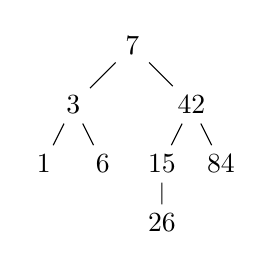
\begin{tikzpicture}[level distance=0.75cm,
  level 1/.style={sibling distance=1.5cm},
  level 2/.style={sibling distance=0.75cm}]
  \node {7}
    child {node {3}
      child {node {1}}
      child {node {6}}
    }
    child {node {42}
      child {node {15}
        child {node {26}}
      }
      child {node {84}}
    };
\end{tikzpicture}
\caption{Example of a Binary Tree}
\label{fig:binarytree}
\end{figure}

The example in Figure~\ref{fig:binarytree} is called a \emph{binary tree} because all nodes have at most two children. 
The top-most node in the tree,~$7$ is called the \emph{root}, which has two children that are trees themselves~$3$ and~$41$. 
The root has a \emph{depth} of zero, whereas~$3$ and~$41$ have depth of one. 
A node~$m$ is a child of node~$a$ if there is a direct edge between~$a$ and~$m$, where the depth level of~$a$ is exactly one fewer than~$m$'s depth level. 
We consider a node~$m$ to be a \emph{descendant} of node~$a$ if there is a sequence of edges from~$a$ to~$m$, where the depth level of~$a$ is at least one fewer than~$m$'s depth level. 
The \emph{height} of a tree~$T$ is the maximum of the depth of~$T$'s root and its children. 
In the example, the tree's height is three due to the path from~$7$ to~$26$.

At this point the reader may await us to show them a collections framework implementation of a tree. 
Unfortunately, Java provides no implementation of trees in its collections framework. 
To compensate, we provide a library that mimics what Java might provide (see~\Cref{appendix-bst-library} for the code implementation). 
In this library we include the \ttt{BinarySearchTree} class, alongside a few other tree implementations that are more complex. 
The difference between a binary search tree and a standard binary tree is that the elements are ordered. 
All nodes to the left of a node~$T$ are ``less than''~$T$, whereas all nodes to the right of~$T$ are greater than~$T$.
The tree example from Figure~\ref{fig:binarytree} is, coincidentally, a binary search tree.

\begin{figure}[tp]
  %\begin{wrapfigure}[25]{r}[0.75in]{0.55\textwidth}
    \small
    \begin{tcolorbox}[title=Teaching Java Binary Search Trees]
      A \emph{binary search tree}\index{binary search tree} is a data structure that stores elements in sorted order.
      \vspace{2ex}
      % \hrule
      % \vspace{2ex}
    \begin{description}
      \item [\ttt{BinarySearchTree<$T$> $t =$ new BinarySearchTree<>$(v)$}] creates a binary search tree~$t$ whose root has the value~$v$.
      \item [\ttt{BinarySearchTree<$T$> $t =$ new BinarySearchTree<>$(v, \mathit{cmp})$}] creates a binary search tree~$t$ whose root has the value~$v$ and uses $\emph{cmp}$ as a comparator when inserting values.
      \item [\ttt{void insert$(v)$}] inserts $v$ into the existing tree using either the stored comparator or the natural ordering of the $T$ type.
      \item [\ttt{BinarySearchTree<$T$> contains$(v)$}] determines whether or not $v$ is in the tree. If so, the subtree where $v$ is the root is returned; \ttt{null} otherwise.
      \item [\ttt{int size$()$}] returns the number of elements in the tree.
      \item [\ttt{BinarySearchTree<$T$> getLeft$()$}] returns the left child of the tree, or \ttt{null} if non-existent.
      \item [\ttt{BinarySearchTree<$T$> getRight$()$}] returns the right child of the tree, or \ttt{null} if non-existent.
      \item [\ttt{BinarySearchTree<$T$> getParent$()$}] returns the parent of the tree, or \ttt{null} if non-existent.
      \item [\ttt{boolean isLeaf$()$}] returns \ttt{true} if this tree has no children, and \ttt{false} otherwise.
      \item [\ttt{boolean isRoot$()$}] returns \ttt{true} if this tree has no parent, and \ttt{false} otherwise.
    \end{description}
  \end{tcolorbox}
    \caption{Useful Binary Search Tree Methods.}
    \label{fig:bstmethods}
  \end{figure}

To create a binary search tree, we initialize and instantiate an object of type \ttt{BinarySearchTree}.\footnote{We do \emph{not} initialize the type to \ttt{Tree} because a \ttt{Tree} does not contain methods for accessing the children of the tree.}
Similar to how \ttt{ArrayList} and \ttt{LinkedList} are ``kinds of'' \ttt{List} objects, a \ttt{BinarySearchTree} is a ``kind of'' \ttt{Tree} object.
To add an element to the binary search tree, we invoke its \ttt{add} method. 
Nodes are inserted according to their natural ordering if a \ttt{Comparator} is not specified when instantiating the binary search tree, identical to priority queues.
Be aware that the elements of the tree must be \ttt{Comparable}.

\myexample{To visit the elements of a binary tree, we can write one of three methods: \ttt{preorderTraversal}, \ttt{inorderTraversal}, or \ttt{postorderTraversal}.}
All three traversal types are recursive by design.
\begin{itemize}
  \item A \emph{preorder traversal} visits the current node, then recurses on its left child, then recurses on its right child.
  \item An \emph{inorder traversal} recurses on its left child, then visits the current node, then recurses on its right child.
  \item A \emph{postorder traversal} recurses on its left child, then recurses on its right child, then visits the current node.
\end{itemize}

Let's design the \ttt{List<T> inorderTraversal(Tree<T> t)} method, which returns a list of the elements in the tree after an inorder traversal. 
An interesting (and mathematically-provable) property of this traversal is that it always visits the elements in sorted order (according to the natural ordering or the comparator). 
To make testing this method easier, we will take advantage of the fact that we can pass a list of values to the \ttt{BinarySearchTree} constructor, which "bulk adds" them to the tree.

%\enlargethispage{-2\baselineskip}
\begin{lstlisting}[language=MyJava]
import static Assertions.assertAll;
import static Assertions.assertEquals;

import java.util.List;
import learningjava.trees.BinarySearchTree;

class InorderTraversalTester {

  @Test
  void testInorderTraversal() {
    BinarySearchTree<Integer> t1 = new BinarySearchTree<>();
    BinarySearchTree<Integer> t2 = new BinarySearchTree<>(List.of(7,42,1,6,15,84,26));
    assertAll(
      () -> assertEquals(List.of(), inorderTraversal(t1)),
      () -> assertEquals(List.of(1, 6, 7, 15, 26, 42, 84), inorderTraversal(t2)));
  }
}

\end{lstlisting}

\newpage
\begin{lstlisting}[language=MyJava]
import java.util.Comparable;
import java.util.List;
import java.util.ArrayList;
import learningjava.trees.Tree;
import learningjava.trees.BinarySearchTree;

class InorderTraversal {

  /**
   * Returns a list of the elements in the tree after an inorder traversal.
   * @param t the tree to traverse.
   * @return a list of elements.
   */
  static <T extends Comparable<T>> List<T> inorder(BinarySearchTree<T> t) {
    if (t == null) { return new ArrayList<>(); } 
    else {
      List<T> left = inorder(t.getLeft());
      List<T> right = inorder(t.getRight());
      List<T> res = new ArrayList<>();
      res.addAll(left);
      res.add(t.getValue());
      res.addAll(right);
      return res;
    }
  }
}
\end{lstlisting}

A tree is said to be \emph{balanced} if the heights of its left and right children differ by at most one.
This property allows for very fast object lookup times, insertions, and removals. 
Maintaining the balance factor of a tree is a non-trivial task, though, and the \ttt{BinarySearchTree} class does not balance the tree, meaning the fast operation times are not guaranteed.
In fact, these operations are, in their worst case, the same as a linked list, because the shape of a \emph{totally unbalanced} binary search tree resembles a list. 
By ``totally unbalanced,'' we mean that all elements are to the left or right of the root, a property that applies recursively to its children.

\myexample{Let's design the \ttt{T findMax(BinarySearchTree t)} method that finds the largest element of a binary search tree. All this involves is following the right-most child until we reach a dead-end. Because all elements to the right of another are larger than the node, this task is trivial.}

\begin{lstlisting}[language=MyJava]
import static Assertions.assertEquals;
import static Assertions.assertAll;

import java.util.List;
import learningjava.trees.BinarySearchTree;

class FindMaxTester {

  @Test
  void testFindMax() {
    BinarySearchTree<Integer> t1 = new BinarySearchTree<>();
    BinarySearchTree<Integer> t2 = new BinarySearchTree<>(List.of(7, 42, 1, 6, 84, 26));
    assertAll(
      () -> assertEquals(null, findMax(t1));
      () -> assertEquals(84, findMax(t2)));
  }
}
\end{lstlisting}

% \enlargethispage{3\baselineskip}
\begin{lstlisting}[language=MyJava]
import java.util.Comparable;
import learningjava.trees.BinarySearchTree;

class FindMax {

  /**
   * Finds the maximum value in a tree.
   * @param t the tree to search.
   * @return the maximum value in the tree, or null if the tree is empty.
   */
  static <T extends Comparable<T>> T findMax(BinarySearchTree<T> t) {
    if (t.isEmpty()) { return null; } 
    else if (t.getRight().isEmpty()) { return t.getValue(); } 
    else { return findMax(t.getRight()); }
  }
}
\end{lstlisting}

\myexample{Let's design the \ttt{boolean isBalanced(Tree t)} method to determine whether or not a tree is balanced.} As we stated, a tree is balanced if the difference between the heights of its left and right subtrees differ by at most one. The idea is to recursively traverse each subtree until we reach a leaf, at which we know that the tree is balanced. We then compare the heights of the left and right subtrees, and if they differ by more than one, we return \ttt{false}. Because we use a logical \ttt{AND} operator, if any subtree is unbalanced, the entire tree is unbalanced, because the \ttt{false} return value propagates upward.

\begin{lstlisting}[language=MyJava]
import static Assertions.assertTrue;
import static Assertions.assertFalse;
import static Assertions.assertAll;

import java.util.List;
import learningjava.trees.BinarySearchTree;

class IsBalancedTester {

  @Test
  void testIsBalanced() {
    BinarySearchTree<Integer> t1 = new BinarySearchTree<>();
    BinarySearchTree<Integer> t2 = new BinarySearchTree<>(List.of(7,42,1,6,15,84,26));
    BinarySearchTree<Integer> t3 = new BinarySearchTree<>(List.of(10, 5, 20));
    assertAll(
      () -> assertTrue(isBalanced(t1)),
      () -> assertFalse(isBalanced(t2)),
      () -> assertTrue(isBalanced(t3)));
  }
}
\end{lstlisting}

%\enlargethispage{6\baselineskip}
\begin{lstlisting}[language=MyJava]
import java.util.Comparable;
import learningjava.trees.BinarySearchTree;

class IsBalanced {

  /**
   * Determines whether a tree is balanced. A tree is balanced if the difference 
   * between the heights of its left and right subtrees differ by at most one.
   * @param t the tree to check.
   * @return true if the tree is balanced, false otherwise.
   */
  static <T extends Comparable<T>> boolean isBalanced(BinarySearchTree<T> t) {
    if (t.isEmpty()) {
      return true;
    } else {
      boolean left = isBalanced(t.getLeft());
      boolean right = isBalanced(t.getRight());
      int leftHeight = t.getLeft().height();
      int rightHeight = t.getRight().height();
      return left && right && Math.abs(leftHeight - rightHeight) <= 1;
    }
  }
}
\end{lstlisting}

\myexample{Let's design the \ttt{BinarySearchTree<T> inorderSucc(BinarySearchTree<T> t)} method, which returns the inorder successor of a node in a given binary search tree.} 
The inorder successor of a node $n$ is the node with the smallest value that is greater than $n$'s value. 
Another way to phrase it is the next-greatest element in the tree.
The algorithm to find the inorder successor of a node $n$ is as follows:
\begin{itemize}
  \item If $n$ has a right child, then the inorder successor is the left-most child of $n$'s right subtree.
  \item If $n$ has no right child, then the inorder successor is the first ancestor of $n$ that is a left child.
\end{itemize}
Following the first case is trivial, because we only need to traverse the left subtree of $n$'s right child. 
The second case is more difficult, because we need to traverse the tree \emph{upwards} until we find the first ancestor that is a left child. 
We can do this by keeping track of the parent of $n$, and if $n$ is its parent's left child, we return the parent.

\begin{lstlisting}[language=MyJava]
import static Assertions.assertAll;
import static Assertions.assertEquals;
import java.util.List;
import learningjava.trees.BinarySearchTree;

class InorderSuccTester {

  @Test
  void testInorderSucc() {
    BinarySearchTree<Integer> t1 = new BinarySearchTree<>();
    BinarySearchTree<Integer> t2 = new BinarySearchTree<>(List.of(7, 42, 1, 6, 84, 26));
    assertAll(
      () -> assertEquals(null, inorderSucc(t1));
      () -> assertEquals(null, inorderSucc(t2.contains(42)));
      () -> assertEquals(15, inorderSucc(t2.contains(7)));
      () -> assertEquals(42, inorderSucc(t2.contains(26))));
  }
}
\end{lstlisting}

\begin{lstlisting}[language=MyJava]
import java.util.Comparable;
import learningjava.trees.BinarySearchTree;

class InorderSuccessor {

  /**
   * Returns the inorder successor of a node in a binary search tree.
   * @param t the node to find the successor of.
   * @return the inorder successor of the node, or null if the node has no successor.
   */
  static <T extends Comparable<T>> T inorderSuccessor(BinarySearchTree<T> t) {
    if (t.isEmpty()) { return null; } 
    else if (t.getRight() != null) {
      BinarySearchTree<T> temp = t.getRight();
      while (temp != null) {
        temp = temp.getLeft();
      }
      return temp;
    } else {
      BinarySearchTree<T> parent = t.getParent();
      while (parent != null && t == parent.getRight()) {
        t = parent;
        parent = parent.getParent();
      }
      return parent;
    }
  }
}
\end{lstlisting}

\myexample{Let's see an example of why we might care about finding the inorder successor of a node.}
We will design the \ttt{Set<T> findBetween(BinarySearchTree<T> t, T min, T max)} method, which returns a set of all elements in the tree that are between \ttt{min} and \ttt{max}. 
There are two ways we can solve this problem: (1) traverse the tree and add elements to the set if they are between \ttt{min} and \ttt{max}, or (2) find the inorder successor of \ttt{min}, and then traverse the tree until we reach \ttt{max}.
The former approach is more straightforward, but the latter is more efficient, because it takes advantage of the fact that the tree is ordered. 
The latter algorithm is as follows:
\begin{itemize}
  \item Find the inorder predecessor to \ttt{min}, or \ttt{min} itself if it is in the tree.
  \item Traverse the tree until we reach \ttt{max}, adding elements to the set as we go, computing the inorder successor of each node.
\end{itemize}

First, we need an algorithm to find the inorder predecessor of a node. 
This encompasses searching for the location of the node in the tree and returning it, if it exists. Otherwise we return the parent of the last node we visited. We will explicitly show the \ttt{findPredecessor} method, but it will be used in the implementation of our \ttt{findBetween} method.

%\enlargethispage{2\baselineskip}
\begin{lstlisting}[language=MyJava]
import static Assertions.assertEquals;
import static Assertions.assertAll;

import learningjava.trees.BinarySearchTree;

class FindBetweenTester {

  @Test
  void testFindBetween() {
    BinarySearchTree<Integer> t1 = new BinarySearchTree<>();
    BinarySearchTree<Integer> t2 = new BinarySearchTree<>(List.of(7, 42, 1, 6, 84, 26));
    assertAll(
      () -> assertEquals(Set.of(), findBetween(t1, 0, 100));
      () -> assertEquals(Set.of(1, 6, 7, 26, 42), findBetween(t2, 0, 100));
      () -> assertEquals(Set.of(6, 7, 26), findBetween(t2, 3, 26));
      () -> assertEquals(Set.of(6, 7), findBetween(t2, 3, 25)));
  }
}
\end{lstlisting}

\newpage
\begin{lstlisting}[language=MyJava]
import java.util.Comparable;
import java.util.HashSet;
import java.util.Set;
import learningjava.trees.BinarySearchTree;

class FindBetween {

  /**
   * Returns a set of all elements in the tree that are between min and max.
   * @param t the tree to search.
   * @param u the minimum value.
   * @param v the maximum value.
   * @return a set of elements between u and v.
   */
  static <T extends Comparable<T>> Set<T> findBetween(BinarySearchTree<T> t, T u, T v) {
    Set<T> res = new HashSet<>();
    BinarySearchTree<T> temp = findPredecessor(t, u);
    while (temp != null && temp.getValue().compareTo(v) <= 0) {
      // Add the element to the set if it is between u and v.
      if (temp.getValue().compareTo(u) >= 0) {
        res.add(temp.getValue());
      }
      temp = inorderSuccessor(temp);
    }
    return res;
  }
}
\end{lstlisting}

Maintaining a balanced binary tree, as we suggested earlier, guarantees fast operations. 
This invariant is non-trivial to maintain, and there are several \emph{height-balancing} tree data structures that do so. 
For example, there are \emph{AVL} trees, \emph{red-black} trees, and \emph{splay} trees (the list is by no means exhaustive)~\Citep{clrs,weissjava}. 
Trees are a natural fit for programming language interpreters and design. Moreover, height-balancing trees are the basis for the \ttt{TreeSet} and \ttt{TreeMap} classes, which guarantee quick operation times.
We end our discussion on trees here, but we will revisit them in a subsequent chapter on advanced object-oriented programming, where their practicality becomes more apparent.